Our system mainly consists of two major parts: image preprocessing and GUI
design. In the following we will describe the concepts generated in both parts.
Fig.\ref{fig:MorphChart} is our morphological chart. Among listed functions,
image augmentation, object detection, human pose estimation and semantic
segmentation belongs to image preprocessing and the rest of them are the part
of GUI design.
\begin{figure}[h!]
  \centering 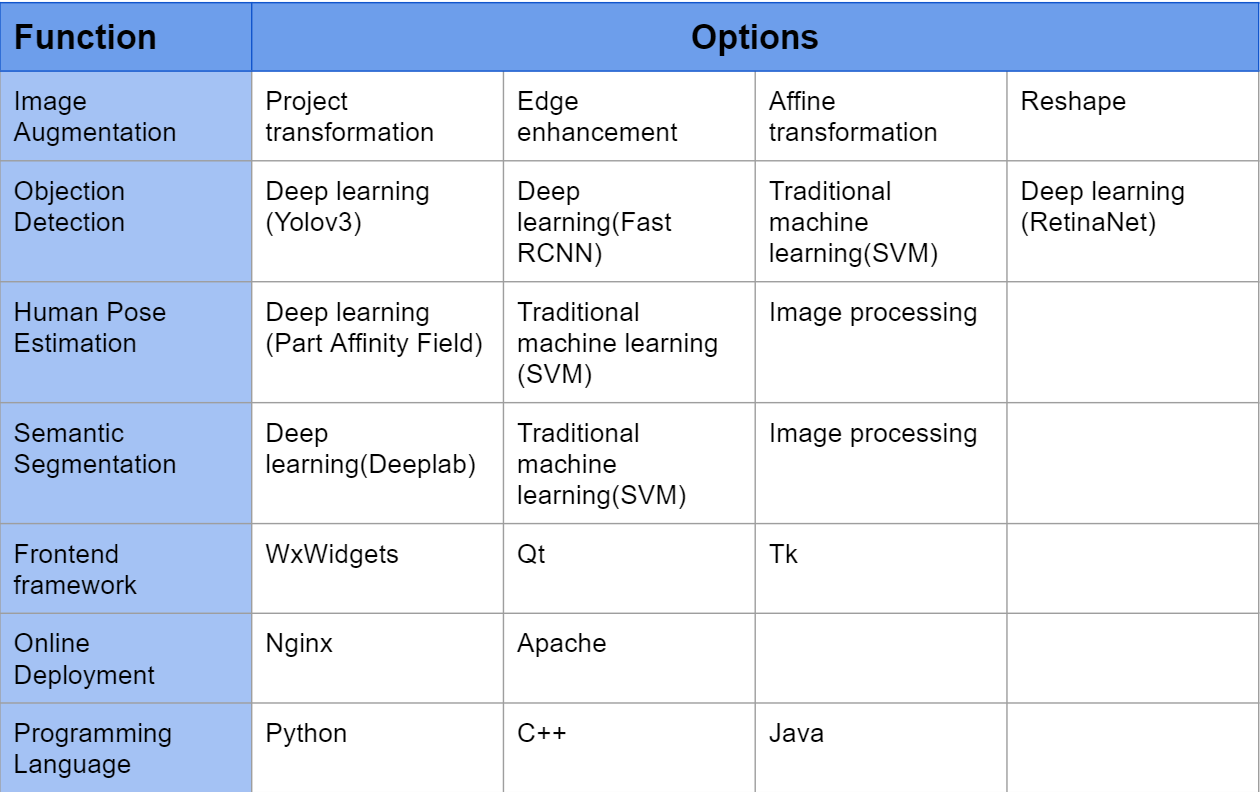
\includegraphics[width=\linewidth]{morp.png}
  \caption{Morphological chart}
  \label{fig:MorphChart}
\end{figure}

\subsection{Image Preprocessing}
We have done the literature research on several image processing methods.
Combining our knowledge on basic machine learning and computer vision
techniques, we come up with three concepts. On one hand, we consider
traditional image processing methods to pre-annotate objects in images. On the
other hand, machining learning offers more functionality and flexibility in
preprocessing. In this category, we consider two concepts: traditional machine
learning and deep learning. Fig. \ref{fig:backend} is our process of concept
generation.
\begin{figure}[h!]
  \centering 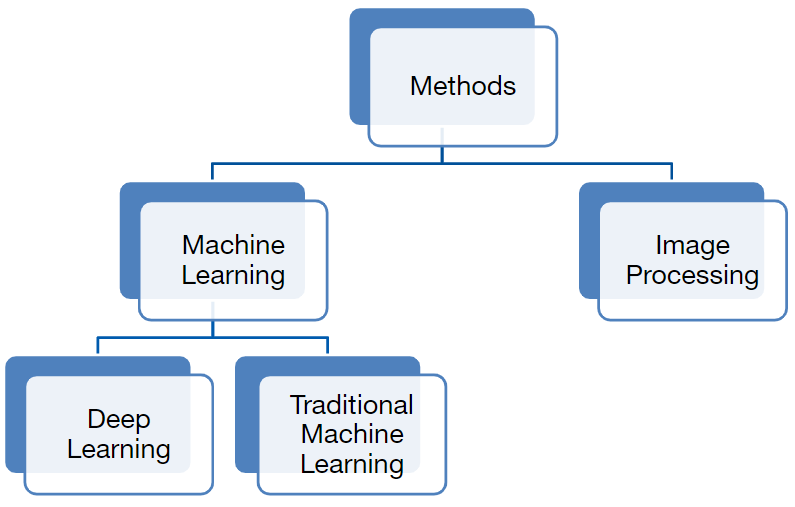
\includegraphics[width=\linewidth]{concept_backend.png}
  \caption{Concept generation of image preprocessing}
  \label{fig:backend}
\end{figure}


\subsection{GUI Design}
For GUI Design, we choose a popular open source GUI libraries, on which we
build our software. Taking portability and code quality into account, after
sifting through various libraries, we select Qt, WxWidgets and Tk as candidates.
